%%%%%%%%%%%%%%%%%%%%%%%%%%%%%%%%%%%%%%%%%%%%%%%%%%%%%%%%%%%%%%%%%%%%%%%%%%%%%%%%
% conclusion.tex:
%%%%%%%%%%%%%%%%%%%%%%%%%%%%%%%%%%%%%%%%%%%%%%%%%%%%%%%%%%%%%%%%%%%%%%%%%%%%%%%%
\chapter{Conclusion and Discussion}
\begin{figure}[!htbp]
    \centering
    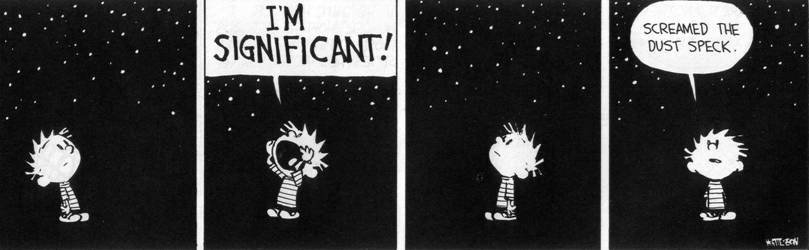
\includegraphics[width=\textwidth]{figures/CalvinAndHobs.jpg}
    \caption[]{Calvin from Calvin and Hobbes tries to deal with his feeling of self worth compared with the scale of the universe\cite{calvinAndHobs}}
    \label{fig:calvin}
\end{figure}{}

The cross-section of the variable \phistar of the \Z boson decay to lepton pairs was measured using 19.7 fb$^{-1}$ of $\sqrt{s}=\SI{8}{TeV}$ data collected with the CMS detector. This data was then unfolded using a \MADGRAPH sample and compared to \POWHEG + \PYTHIAeight samples, using different ``tunes".

All \POWHEG + \PYTHIAeight tunes match unfolded data within 5\%  for $\phistar<0.2$ and are practically identical for higher \phistar. For $\phistar<0.03$, smaller values of either $\SigmaHard$ or $\SigmaSoft$ decreased the disagreement between data and theory. This was expected since lowering either variable results in a smaller \bosonpt of the \Z and reduces the deficit of low \bosonpt \Z bosons. However, major changes of the tune, e.g. decreasing both $\SigmaHard$ and $\SigmaSoft$ by a factor of two, were unable to completely remove the disagreement. It therefore does not appear to be possible to remove the disagreement between theory and data at low \phistar by making a reasonable change in either $\SigmaHard$ or $\SigmaSoft$. It also appeared that the for medium \phistar region($0.03<\phistar<0.15$) lowering $\SigmaHard$ or $\SigmaSoft$  increased the disagreement. For high \phistar the tune has a trivial effect with all tunes overestimating the cross-section by the same amount within uncertainty. Therefore it does not appear that the variables $\SigmaHard$ or $\SigmaSoft$ are responsible for the disagreement between data and theory. There are however many other free parameters used by \PYTHIAeight that could possibly be partially responsible for the disagreements between data and theory, such as the PDF used which could be studied by another analysis in the future. Attempting to find settings in the hadronizer that remove the disagreement between data and theory of \phistar are important in lowering the uncertainty of the W mass measurement. Overall it is important to study this disagreement since if the hadronizer is not at fault it could imply a problem with the Standard Model. Therefore, in the future it is important that studies attempt to find the reason for the difference between theory and data, and if possible if it.
\label{conclusion_chapter}
%%%%%%%%%%%%%%%%%%%%%%%%%%%%%%%%%%%%%%%%%%%%%%%%%%%%%%%%%%%%%%%%%%%%%%%%%%%%%%%%

%%%%%%%%%%%%%%%%%%%%%%%%%%%%%%%%%%%%%%%%%%%%%%%%%%%%%%%%%%%%%%%%%%%%%%%%%%%%%%%%
